
\section{Luck}
\andyc{Lucas's section}
\lucasc{I like this Quote from Will C. I found while searching the forum for the basketball tourney. I think it fits too. }
\noindent No change. It's not about the prize, it's the element of luck involved that makes it 50\%.\\
\noindent  William Cukierski ,Kaggle Competition Admin \\

Previously we have detailed popular methods for prediction and outlined our new methodology that accounts for specific match ups. In final component of this paper, we address the high degree of chance present in NCAA tournaments and consequently prediction for NCAA tournaments.  Specifically, we address sensitivity in a Kaggle style leader board. It's natural to think 2nd place almost won, but how close was 20th place to winning? 

% some verbiage in here... 

To study the effect of luck we take the idea that the 2nd place team almost won and we attempt to quantify `almost.' To that end, we examine alternate realities where a losing team in an overtime game is treated instead as a winning team. We focus only on overtime games because it seems most reasonable to think of the losing team as having won in those cases. Recall that the loss function used for scoring of the waggle competition is

\begin{equation}
\sum_{i=1}^n\frac{y_ilog(p_i)+ (1-y_i)log(1-p_i)}{n},
\end{equation}

Where $y_i$ is a binary variable taking value 1 when the team wins and 0 otherwise and $0 \leq p_i \leq 1$ denotes the predicted value for the team in the $i$th game. We consider how dependent the rankings of individual teams are on the characteristics of this particular loss function. To answer this question we studied a couple of possible alternate scoring functions. We consider the following scoring functions: 
 
\begin{equation}\label{eqn:first_score_function}
-log(1-2|.5-p_i|)
\end{equation} 

\begin{equation}\label{eqn:second_score_function}
-log(1-|.5-p_i|)
\end{equation} 

\begin{equation}\label{eqn:third_score_function}
-log(1-|y_i-p_i|)
\end{equation} 
Here, for brevity, we only write the part of the loss function multiplied by the $(1-y_i)$ term. Moreover, in Function \ref{eqn:third_score_function}, $y_i \in \{0,.5,1\}$, where now the $0.5$ is the realized value when teams go into overtime. Figure \ref{fig:scoring_functions} is a plot of the different score functions for values $0\leq p_i \leq 1$.  

\begin{figure}[h]
\centering
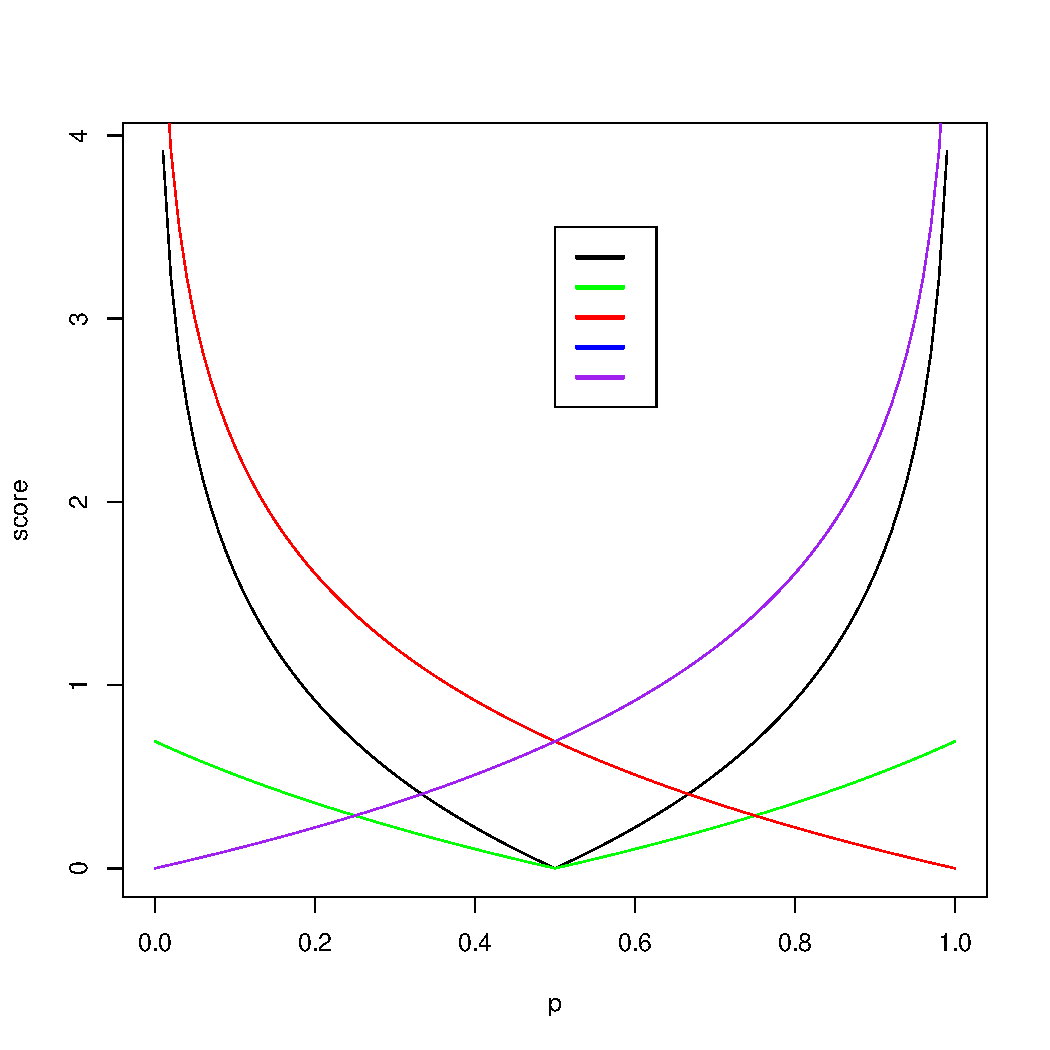
\includegraphics[width=.7\textwidth]{loss_function_plot.pdf}
\caption{A plot of the various loss functions as a function of the prediction $p_i$.  }
\label{fig:scoring_functions}
\end{figure}

It is clear from looking at Figure \ref{fig:scoring_functions} that the different scoring functions treat the contestants (IAN: should this be contestant's?) confidence differently. Both the first and the second score function are symmetric about 0.5 which is aesthetically pleasing. Moreover, the first score function penalizes much more for confident predictions than the second. 

One might wonder, given the plethora of choices one might use to rank contestants, how much is a result of a specific function and how much hold sir we move from one scoring function to another?(IAN: I'm not sure what you're getting at in the previous sentence. How much of what is a result of a specific function?) To examine this, we made a plot of the contestant predictions scored under the various loss functions described above. The results of this plot are shown in Figure \ref{fig:score_rank_plot}. 

  \begin{figure}[h]
\centering
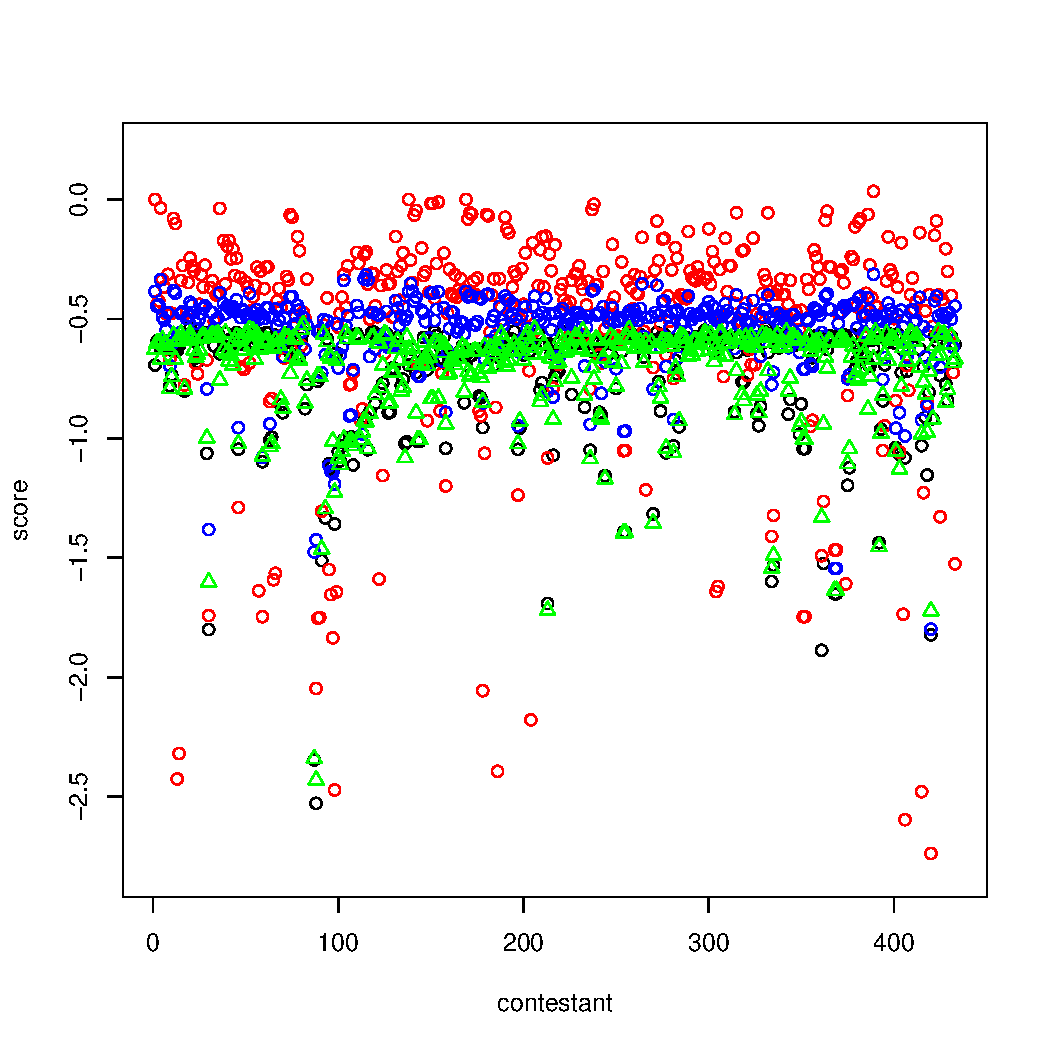
\includegraphics[width=.7\textwidth]{prelim_rank_plot.pdf}
\caption{The scores of each contestant under the different loss functions. A smaller score is better.  }
\label{fig:score_rank_plot}
\end{figure}

\lucasc{Now the concluding paragraph for section}

While much has been made in contest forums and in books \cite{schutt2013doing} about leakage and how leakage is often exploited to win competitions, it is somewhat refreshing to see that other choices play little, if any, into the ultimate results of a competition. While luck ultimately plays a role in the basketball games themselves and the results of prediction tournaments, some players are able to consistently outperform. These consistent performs are lucky, but lucky in the sense they are endowed with particular gifts that the rest of us mortals only dream of and practice in hopes of achieving some semblance of success.  